\chapter{Motivation:What are special functions?}
\label{ch:motivation}


In elementary mathematics we are used to work with a very limited set functions that we call \idxentry{elementary functions}{functions!elementary}{elementary-function}{elementary}. Essentially, elementary functions are $x^\alpha$ for $\alpha\in\Real$, trigonometric function and their inverses, exponential and logarithm, and finite combinations of them obtained by addition, subtraction, multiplication, division
or composition. 

Although this set of functions is very restrictive, they were chosen as elementary because they appear in many contexts in both mathematics and physics and they can solve a surprisingly rich set of problems. Results
of integrals or solutions that can be written in terms of elementary functions are considered as "nice". In such case we say that given problem admits a solution in a \idxentry{closed form}{solution!closed form}{closed-form-sol}{closed form}.

Nevertheless, there is no reason to expect that {\itshape every} problem will be solvable in terms of elementary functions. Indeed, it is a well-known example that the integral
\begin{align}\label{eq:F}
    F(x) &= \int_{0}^x e^{-u^2}\,\dd u
\end{align}
cannot be expressed in terms of elementary functions\footnote{We have chosen the lower limit to $0$ just for convenience, the point is that the primitive function to $e^{-x^2}$ is not elementary.}. Still, function $F$ introduced by \eqref{eq:F} is a well-defined function, since the integrand is continuous on $\Real$ (piece-wise continuity would suffice), it is just not an elementary function. 

Formally, we can find a solution, for example, in the form of \idxentry{Taylor expansion}{expansion!Taylor}{taylor-expansion}{Taylor}. Recall that the \idxentry{Taylor expansion of the exponential function
}{expansion!Taylor!exponential}{taylor-expansion-expfunc}{exponential}  is
\begin{align}\label{eq:Taylor-exp}
    e^x &= \sum_{n=0}^\infty \frac{x^n}{n!}\, ,
\end{align}
so that 
\begin{align}\label{eq:Taylor-F}
    F(x) &= \sum_{n=0}^\infty\frac{(-1)^n}{n!}\int_0^x u^{2\,n}\,\dd u =
        \sum_{n=0}^\infty\frac{(-1)^n}{n!}\,\frac{x^{2\,n+1}}{2\,n+1}\, .
\end{align}
We leave the question of convergence aside but illustrate the result on numerical code in Python. Result \eqref{eq:Taylor-F} is said to be in a \idxentry{non-closed form}{solution!non-closed form}{non-closed-sol}{non-closed form}, because it is expressed as an infinite series which does not sum up to any elementary function. Therefore, solution \eqref{eq:Taylor-F} is the most explicit analytic form of the integral \eqref{eq:F}. 

Let us define the function $\widetilde{F}(x,n_{\max)})$ by
\begin{align}\label{eq:F-tilde}
    \widetilde{F}(x, n_{\max}) &= \sum_{n=0}^{n_{\max}}\,\frac{(-1)^n}{n!}\,\frac{x^{2\,n+1}}{2\,n+1}\, ,
\end{align}
which contains only finitely many terms in the sum. The radius of convergence of series \eqref{eq:Taylor-F} should be infinite so let us find empirically how many terms we need to achieve reasonable accuracy. 

First, in Figure \ref{fig:F}  we plot function $F(x)$ itself obtaining its values by numerical integration which we will now consider as the "exact solution". Next, in Figure \ref{fig:F-tilde} we show graphs of partial sums for values $n_{\max}$ indicated in the title of the figure. We see that the for low values of $n_{\max}$ the sums quickly diverge from the correct limit $\sqrt{\pi}/2$. Qualitatively, the reason is obvious. In order to get infinite radius of the convergence of the Taylor series \eqref{eq:Taylor-F} we need to sum infinitely many terms. Choosing relatively small $n_{\max}$ we still get a polynomial of high degree which quickly diverges. Hence, these divergent terms must be cancelled by higher order terms of the series and we need to sum much more terms in order to achieve desired accuracy. 

\begin{figure}
    \centering
    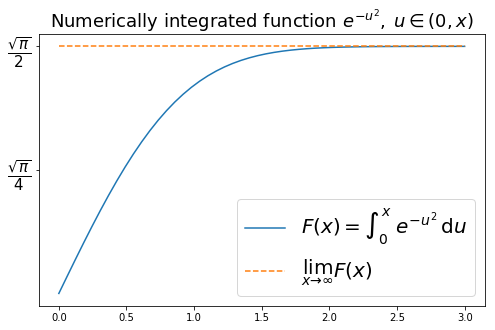
\includegraphics[width=0.7\textwidth]{function-F.png}
        \caption{Function $F(x)$ defined by \eqref{eq:F} obtained by numerical integration in Python. It can be shown {\itshape exactly} that $\lim\limits_{x \to \infty} F(x) = \sqrt{\pi}/2$.}
    \label{fig:F}
\end{figure}

\begin{figure}
    \centering
    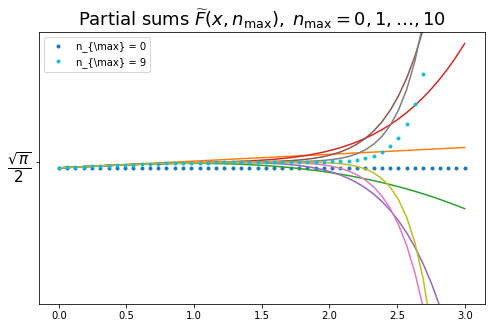
\includegraphics[width=0.7\textwidth]{function-F-tilde.png}
        \caption{Function $\widetilde{F}(x,n_{\max})$ defined by \eqref{eq:F-tilde} obtained by performing actually the sum for indicated values of $n_{\max}$.}
    \label{fig:F-tilde}
\end{figure}

To conclude this line of thoughts, some integrals or differential equations (or even other problems) do not admit a solution in the closed form. Can we consider solution in the form of infinite series \eqref{eq:Taylor-F} as a true, useful solution?

Well, one should realize that even many elementary functions can be, in fact calculated from the series of such kind, except for integer powers $x^n$. We are very familiar with sine or cosine because they have a good geometrical meaning and have been studied a lot, but in order to calculate, say $\sin 1.1$ we cannot resort directly to this geometrical meaning but we have to find the closest value to $1.1$ for which we can derive the value of sine geometrically and then perform a Taylor expansion around this point to reach $x=1.1$ with sufficient accuracy\footnote{Of course, in principle we can calculate {\itshape any value} $\sin x$ by expanding sine about zero, but then we have to sum up too many terms to make the method efficient and sufficiently precise.}.

Hence, our intuitive understanding of meaning of elementary function is important but otherwise it is just a kind of illusion that they are different from special functions like \eqref{eq:Taylor-F}. 

Moreover, also certain special functions appear in the context of physics or mathematics repetitively. \idxentry{Spherical harmonic functions}{functions!harmonic!spherical}{spherical-harmonics}{spherical} appear naturally in problems with spherical symmetry{symmetry!spherical} like the angular part of \Schr equation{equation!\Schr} with spherical potential, in the study of rotational group{group!rotational}, adding angular momenta in quantum mechanics \idxentry{Fourier analysis}{Fourier!analysis}{fourier-analysis}{analysis} of the cosmic microwave background{cosmic microwave background}, etc. \idxentry{Bessel functions}{functions!Bessel}{bessel-functions}{Bessel} are typical for problems with \idxentry{cylindrical symmetry}{symmetry!cylindrical}{cylindrical-symmetry}{cylindrical} (transfer of electromagnetic waves or heat in cylindrical objects) or with \idxentry{helical symmetry}{symmetry!helical}{helical-symmetry}{helical} like DNA. \idxentry{Hypergeometric functions}{functions!hypergeometric}{hypergeom-functions}{hypergeometric} appear in \idxentry{statistics}{statistics}{statistics}{statistics}, in the integrals representing the \idxentry{Feynman diagrams}{Feynman!diagrams}{feyman-diags}{diagrams}.

\idxentry{Special functions}{functions!special}{special-functions}{special} are functions which are not \idxentry{elementary}{functions!elementary}{elementary-function}{elementary}. However, we often use for \idxentry{Fourier series}{Fourier!series}{fourier-series}{series} functions which are in fact elementary but nevertheless call them special. For example, \idxentry{Legendre}{polynomials!Legendre}{legendre-polynomials}{Legendre} or \idxentry{Hermite}{polynomials!Hermite}{hermite-polynomials}{Hermite} are just pure polynomials of finite order. Such polynomials, if they solve the \idxentry{Sturm-Liouville problem}{problem!Sturm-Liouville}{SL-problem}{Sturm-Liouville}, form a \idxentry{complete}{set!complete}{complete-set}{complete} \idxentry{orthonormal}{set!orthonormal}{orthonormal-set}{orthonormal} of functions, meaning that any suitable function can be expanded into the (infinite) Fourier series of such polynomials. In contrast, polynomials $x^n$ do not have this property. Although any function can be expanded into a Taylor series, so that polynomials $x^n$ form a complete set, they are not orthogonal in any meaningful sense. The notion of orthogonality requires the presence of an additional structure, either \idxentry{norm}{norm}{norm}{norm} or \idxentry{inner product}{product!inner}{inner-product}{inner} and polynomials $x^n$ are not equipped with such structures. For these reasons we will call also orthogonal polynomials (like \idxentry{Legendre polynomials}{polynomials!Legendre}{legendre-polynomials}{Legendre}) special functions, although they are just ordinary elementary functions. 
